\documentclass[12pt]{article}
\usepackage{amssymb}
\usepackage[UTF8]{ctex}
\usepackage{geometry}
\usepackage{units}
\usepackage{pifont}
\geometry{
	a4paper,
	total={150mm,237mm},
	left=30mm,
	top=27mm,
	}
\usepackage{amsmath}
\usepackage{enumerate}
\usepackage{lipsum}
\usepackage{graphicx}
\usepackage{hyperref}
\usepackage{indentfirst}
\usepackage[graphicx]{realboxes}
\usepackage{booktabs}
\usepackage{cases}
\usepackage{subfig}  
\usepackage{float}
\usepackage{pythonhighlight}

\setlength{\parindent}{2em}
\title{HW9}
\author{姓名:陈锐林,学号:21307130148}

\begin{document}
\maketitle
\begin{large}
    \noindent Question1\par
\end{large}
这题要补全fork-join.c,根据题目和代码信息;我们要设置信号量,让输出顺序正常(parent => child => parent),通过在child
中sleep来保证正确。所以设置信号量的思路即:parent中wait,child完成并post。代码和运行效果如下:
\begin{figure}[!h]
    \centering
    \subfloat[child]{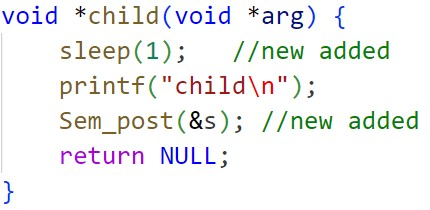
\includegraphics[width=5cm,height=3cm]{hw9-1.jpg} \label{X}}
    \hfill
    \subfloat[parent(main)]{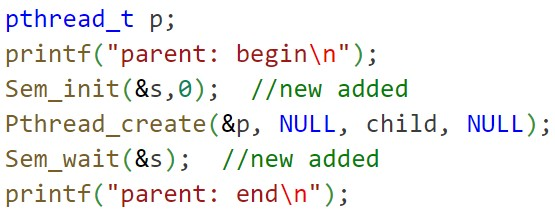
\includegraphics[width=7cm,height=3cm]{hw9-2.jpg} \label{Y}}
\end{figure}
\begin{figure}[h]
    \centering
    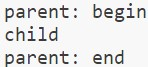
\includegraphics[width=3cm,height=2cm]{hw9-3.jpg}
\end{figure}\\
\begin{large}
    \noindent Question2\par
\end{large}
这题要求实现,每个线程都要在另一个进来之后才能退出。题目也提示了要使用两个信号量;那么就简单了。分别用两个信号量控制两个child。对于
child1,每当开始工作时,post child2的信号量;并等待child2 post自己的信号量;child2类似。这里给出代码(main函数初始化,略去)和运行效果:
\begin{figure}[h]
    \centering
    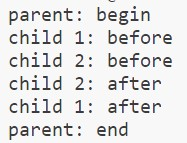
\includegraphics[width=3cm,height=2cm]{hw9-4.jpg}
\end{figure}
\newpage
\begin{figure}[h]
    \centering
    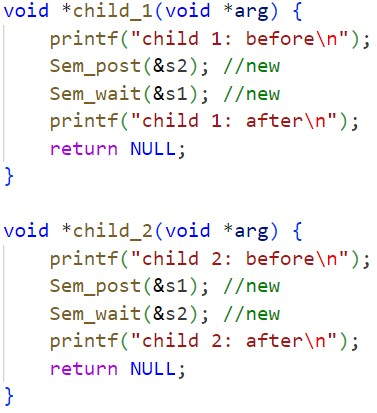
\includegraphics[width=5cm,height=6cm]{hw9-5.jpg}
\end{figure}
\begin{large}
    \noindent Question3\par
\end{large}
这里要实现barrier相关的事务;要求达成的效果是在给定线程数的情况下,先对所有线程做事情A,再做事情B。为了实现该代码,我们需要在barrier中保存线程数,当前等到的线程数。对于某个线程,我们可以对
当前等到的线程数作判断;如果总数不达标,就要调用wait等待。当总数够了,就post。综上,我设置了信号量t1,t2;总线程数N,当前队列内线程数q。t1用来实现等待所有线程进队,t2用来保证对q的更新不会出错。
还需要说明初始化,q和N不必多说;t1该是0,因为要保证从第一个线程开始就等待;t2该是1,保证每次对q的更新都顺利进行并及时post回去。代码和运行(./barrier 2)结果如下:
\begin{figure}[!h]
    \centering
    \subfloat[结构定义和初始化]{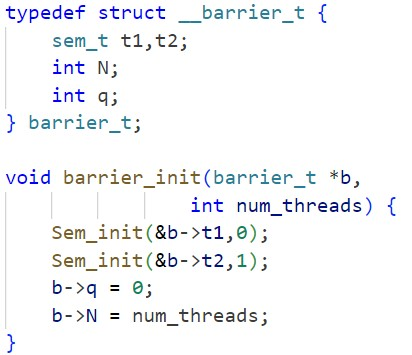
\includegraphics[width=6cm,height=6cm]{hw9-7.jpg} \label{X}}
    \hfill
    \subfloat[函数barrier]{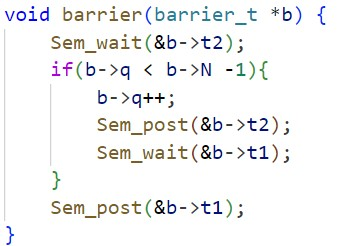
\includegraphics[width=6cm,height=4.5cm]{hw9-8.jpg} \label{Y}}
\end{figure}
\begin{figure}[h]
    \centering
    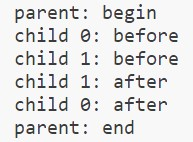
\includegraphics[width=2cm,height=2.7cm]{hw9-6.jpg}
\end{figure}
\newpage
\begin{large}
    \noindent Question4\par
\end{large}
(1)参照前面的内容,可以较容易地实现。用readers表示读者数,为了保证更新的正确,需要一个信号量count;为了保证写的唯一,需要信号量write。为了解决冲突,构造读者优先锁,读者获取锁时,如果他是当前第一个在读的,那就要将write占用;读者释放锁时,
如果当前只剩他一人了,就要及时放开锁。其他就是维护readers,写者正常的wait和post。
(2)饿死的情况是很有可能发生的,如果先进来俩个读者,他们赖着不走;这样无论之后来了多少写者,write将一直为0,写者难以正常写。如下面的例子,明明是两个循环,但是读者只能读到0。
(3)代码(额外添加的sleep没显示)和执行(./reader writer 3 2 2)结果如下:
\begin{figure}[!h]
    \centering
    \subfloat[part1]{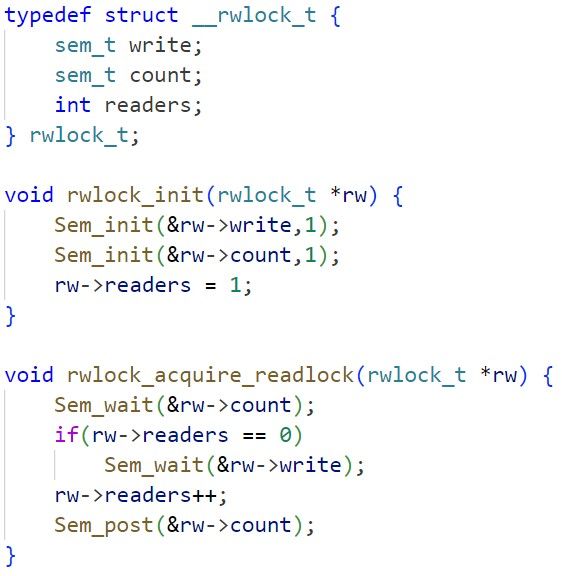
\includegraphics[width=7cm,height=7cm]{hw9-10.jpg} \label{X}}
    \hfill
    \subfloat[part2]{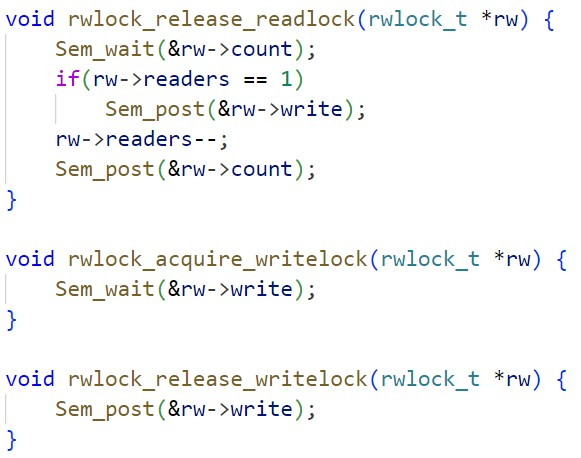
\includegraphics[width=7cm,height=5.5cm]{hw9-11.jpg} \label{Y}}
\end{figure}
\begin{figure}[h]
    \centering
    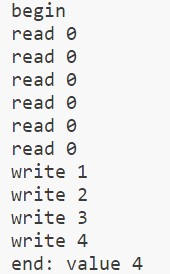
\includegraphics[width=3cm,height=6cm]{hw9-9.jpg}
\end{figure}
\newpage
\begin{large}
    \noindent Question5\par
\end{large}
我们能看到,上面的问题主要是因为读者对写锁write的无条件霸占。所以从这点出发,为了让写者可以有作用,我们可以储存排队要写的人的数量,并在读者尝试上锁时判断是不是还有人要写。自然而然,writers变量的维护也需要一个信息量wcount。读者现在流程就变成:
上锁时,如果有写者在排队,那就要及时让出位置(post wcount和write,再wait read和write);接着再做和之前类似的事。读者的释放操作可以保持不变,即使post write就好。对于写者的操作也有较大变化,当一个写者进来时,首先要对writers进行维护,紧接着要刺探是不是能写(wait write),
写完了要及时把writers复原;写者释放时也还需要post read。代码和运行(和上面一样的命令)截图如下:
\begin{figure}[!h]
    \centering
    \subfloat[part1]{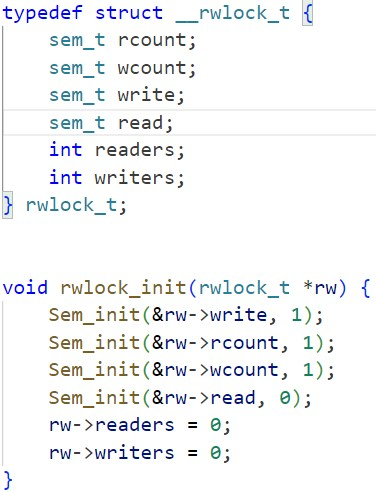
\includegraphics[width=6cm,height=6cm]{hw9-12.jpg} \label{X}}
    \hfill
    \subfloat[part2]{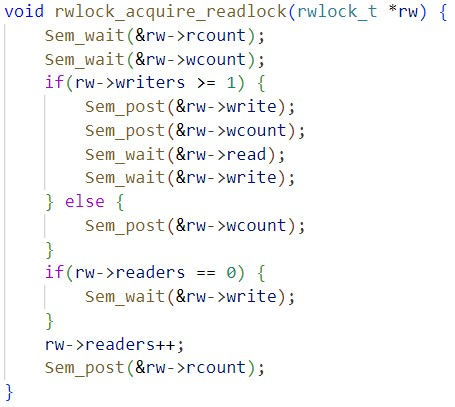
\includegraphics[width=7cm,height=5.5cm]{hw9-13.jpg} \label{Y}}
\end{figure}
\begin{figure}[!h]
    \centering
    \subfloat[part3]{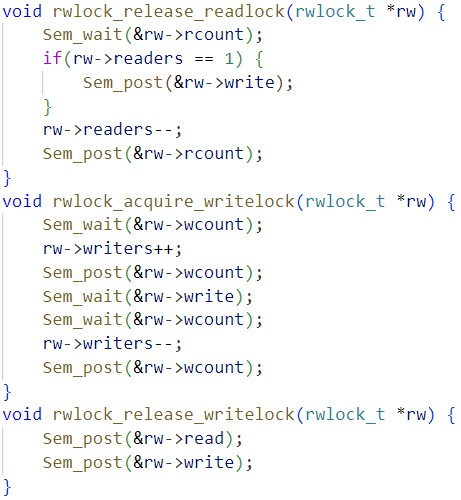
\includegraphics[width=6cm,height=7cm]{hw9-14.jpg} \label{X}}
    \hfill
    \subfloat[part4]{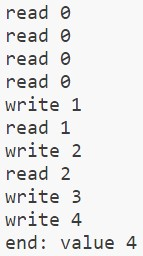
\includegraphics[width=3cm,height=6cm]{hw9-15.jpg} \label{Y}}
\end{figure}
\newpage
\begin{large}
    \noindent Question6\par
\end{large}
只要能保证每个线程都能得到锁并进行正常的工作就行。首先解决怎么展示锁被正常使用,这里直接调用函数pthread\_self()函数展示被锁前后的线程ID即可,会发现输出是正常且对应的。
说回到设计,我主要是用了两个信号量和一个标志。标志value用来指示目前状态;锁被占用,value减小,释放则增大。可以看到,为了避免饥饿,在锁释放时对value判断,如果value还小于0,说明还有
线程卡在了等待阶段。信号量是mutex和turn,初始化为1/0;首个进程可顺利进行,无需关心turn。在acquire阶段,mutex作总体控制,保证value不会发生问题;但如value小于0,在acquire阶段,该线程就等待turn,直到拿到锁;
这是和上面release阶段对应的。代码和运行效果如下:
\begin{figure}[!h]
    \centering
    \subfloat[part1]{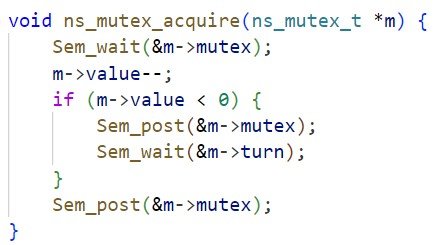
\includegraphics[width=7cm,height=6cm]{hw9-17.jpg} \label{X}}
    \hfill
    \subfloat[part2]{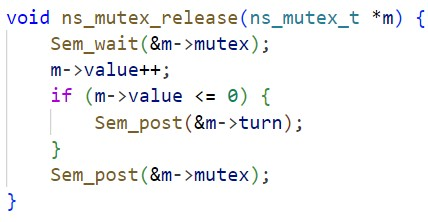
\includegraphics[width=7cm,height=6cm]{hw9-18.jpg} \label{Y}}
\end{figure}
\begin{figure}[!h]
    \centering
    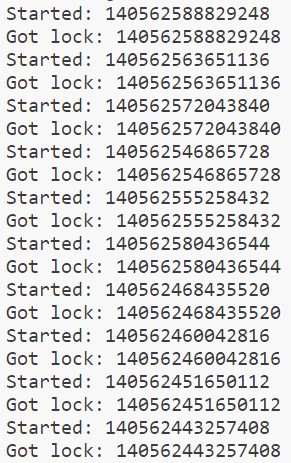
\includegraphics[width=5cm,height=8cm]{hw9-16.jpg}
\end{figure}
\end{document}